\documentclass[12pt,twocolumn]{article}

\usepackage[letterpaper, margin=0.75in]{geometry}
\usepackage{tikz}
\usepackage{graphicx}
\usepackage{caption}
\usepackage{subcaption}
\usepackage{hyperref}
\usepackage{tabularx}
\usepackage{amssymb}
\usepackage{mathtools}
\usepackage{algorithm}
\usepackage{algpseudocode}
\usepackage[english]{babel}
\usepackage[utf8]{inputenc}
\usepackage{flushend}

\renewcommand{\baselinestretch}{0.95}

\title{Reproducing the Results of\\``Distributed Denial of Service Attacks''}
\author{Ashkan Aghdai}

\begin{document}
\maketitle

\begin{abstract}

Here we reproduce Figures \hyperref[fig4]{4} and \hyperref[fig5]{5} of Distributed Denial of Service Attacks paper.
The objective of this experiment is to show how effective Distributed Denial of Service (DDoS) attacks are under two different queuing schemes: Drop Tail and Random Early Detection.
It shows whether or not legitimate users can obtain desired service while a DDoS attack is in process.
Results are verified using a GENI testbed.
\end{abstract}

\begin{figure}[b!]
    \centering
    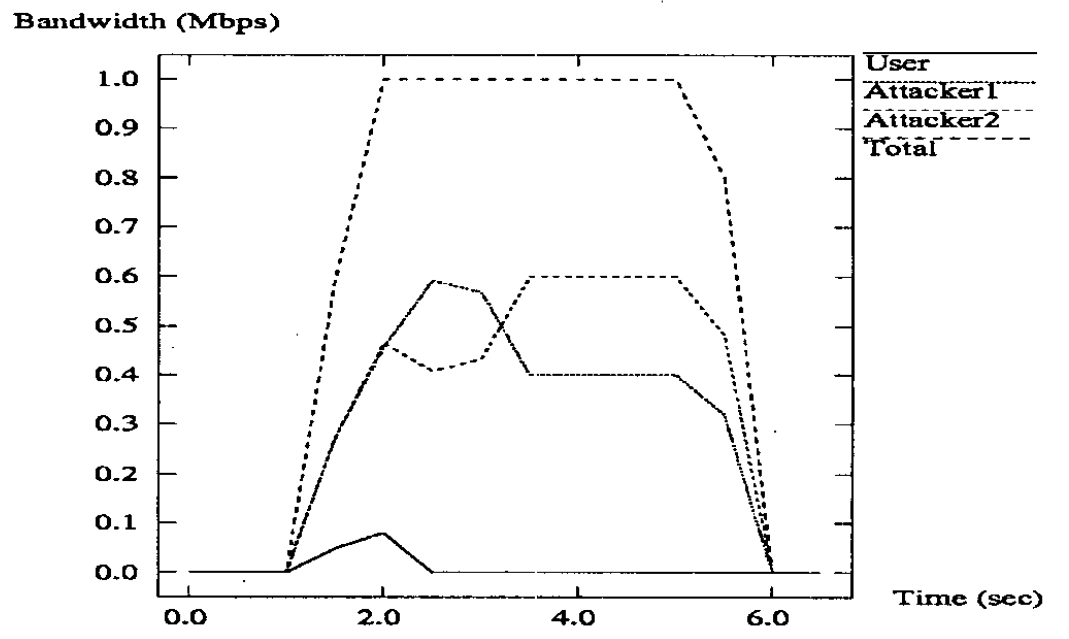
\includegraphics[width=0.45\textwidth]{../Figures/fig4.png} \caption{User's bandwidth during the attack using a DropTail queue \cite{bertsekas1992data}, Figure 4 of \cite{lau2000distributed}.} \label{fig4}
\end{figure}

\begin{figure}[b!]
    \centering
    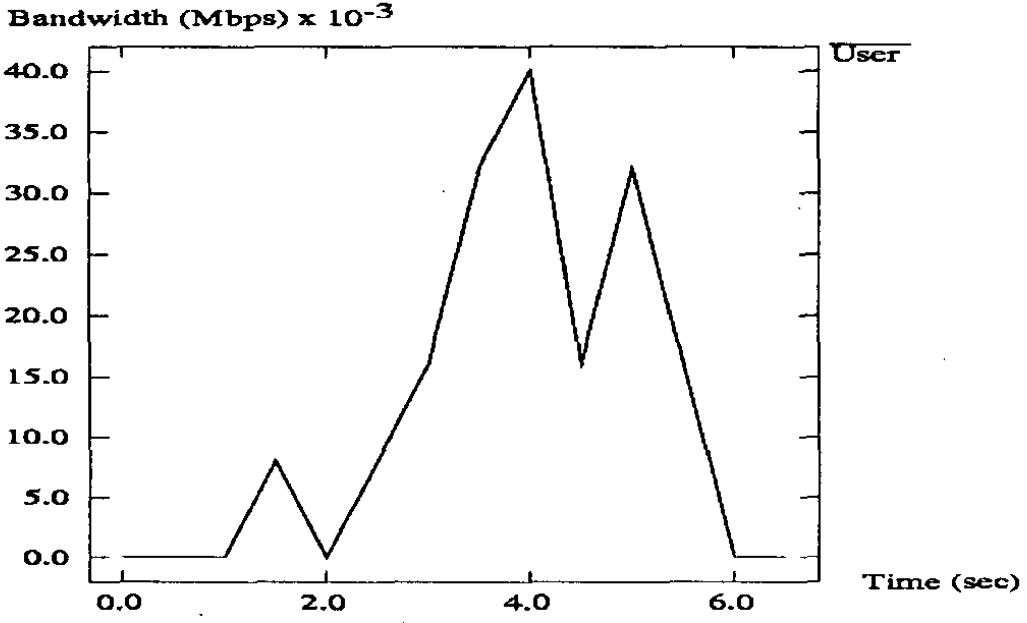
\includegraphics[width=0.45\textwidth]{../Figures/fig5.png} \caption{User's bandwidth during the attack using a RED queue \cite{floyd1993random}, Figure 5 of \cite{lau2000distributed}.} \label{fig5}
\end{figure}

\section{Introduction}

A Denial of Service (DoS) attack is defined as an attempt to make a machine or a resource unavailable to its legitimate users \cite{bellovin1989security}.
When we have more than one source attacking the target, it is called a Distributed DoS (DDoS) \cite{lau2000distributed}.
Typically, attackers try to take control of a lot of unique IP addresses (Zombie Machines) and use them to exhaust a resource either on the target machine, or the network that connects legitimate users to the target machine/s.

\begin{figure}
    \centering
    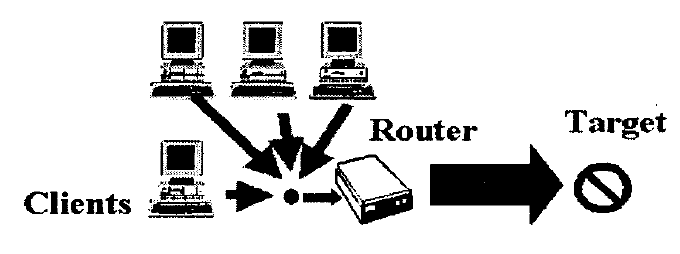
\includegraphics[width=0.35\textwidth]{../Figures/sample.png} \caption{A simple DDoS attack \cite{lau2000distributed}.} \label{sampleDDoS}
\end{figure}

In this experiment, we perform a simple DDoS attack.
As shown in Figure~\ref{sampleDDoS}, a client tries to reach a service through a single hop network with a router connecting it to the server.
Assuming that an attacker takes control of a set of zombie machines connected to the same router, we simulate how he/she can make the service unavailable to the client by targeting the router and overwhelming its queue.
As an outcome, packets will be drooped while the attack is in progress and the client will experience a considerable drop in its bandwidth.
Therefore, the key metric in this experiment is the rate at which client communicates with the server while the attack is in progress.
A rate of zero indicates no connectivity and a rate drop indicates service degradation.

Original results on the paper are acquired from a NS2 simulation.
Here, we reproduce them with GENI testbed.

\section {Experiment Design}

Similar to the original experiment, the client establishes a constant bit rate (CBR) UDP stream to the server.
To verify Figure 4, we show that only 2 zombie machines, as in the figure \ref{arch1}, sending CBR traffic is sufficient to disrupt the service when router implements DropTail queuing policy.
Figure 5 shows how queues with Random Early Detection (RED) policy perform under a DDoS attack.
However, in this scenario we need more zombie machines, as in figure \ref{arch2}, to disrupt the service.
Results from the original paper show that unlike DropTail, the client rate will be decreased rather than going down to zero.
It is still considered to be a successful attack as the client experience noticeable service degradation.

\begin{figure}[b]
    \centering
    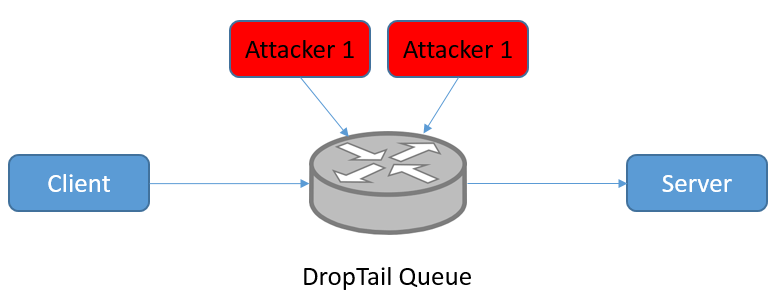
\includegraphics[width=0.5\textwidth]{../Figures/arch1.png} \caption{Architecture for DropTail queue.} \label{arch1}
\end{figure}

\subsection{Choosing the Right Parameters}

Since the authors have not specified the parameters, setting the proper parameters is the toughest part for this project especially for the second part where we experiment with RED, since configuring RED is known to be difficult when it comes to setting proper parameters \cite{floyd1993random}.

\subsubsection{Token Bucket Filter}

\begin{table}
    \centering
    \begin{tabularx}{0.5\textwidth}{X|X|X}
        Parameter & TBF & RED \\
        \hline
        \hline
        Number of Attackers & 2 & 12 \\
        Total Attack Bandwidth & 1.2Mbps & 9Mbps \\
        Queue Size & 550 & 10000 \\
        $min_{th}$ & N.A. & 2500 \\
        $max_{th}$ & N.A. & 7500 \\
        $max_p$ & N.A. & 0.1 \\
        $w_q$ & N.A. & 0.002 \\
        Client's Desired Rate & 0.1Mbps & 0.1Mbps \\
    \end{tabularx}
    \caption{Related parameters.}\label{tt}
\end{table}

For the DropTail queue, we know that the queue rate should be smaller than sum of the clients and two attackers’ rate.
Therefore, I chose CBR rates 0.1Mbps for client and 0.6Mbps for zombie machines using 500B packets all of which to be aggregated on a queue with rate 1Mbps.
As a rule of a thumb queue length is assigned to be at lease as large as the bandwidth delay product (assuming 1ms RTT): $1Mbps*1ms=1Kb=125B$, however, in order for Linux's Token Bucket Filter to work, the queue size should be at least as large as the largest packet. So, in the experiment I have set it to 550 Bytes.
Burst packet size parameter for TBF is also set to 550 bytes, since the incoming traffic is CBR, we do not experience bursts and this parameter does not matter.

\begin{figure}[b]
    \centering
    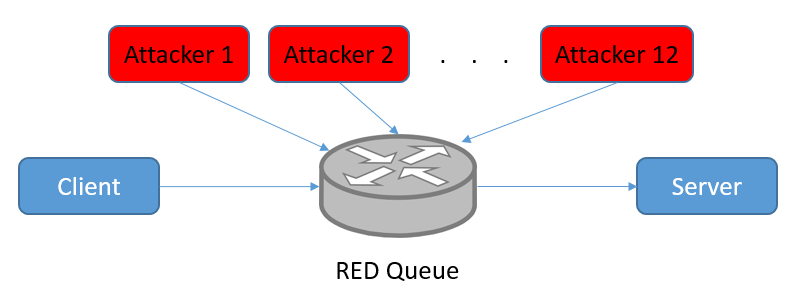
\includegraphics[width=0.5\textwidth]{../Figures/arch2.png} \caption{Architecture for RED queue.} \label{arch2}
\end{figure}

\subsubsection{Random Early Detection}

For RED experiment, we have to set 5 parameters: buffer space, $min_{th}$, $max_{th}$, $max_p$, and $w_q$.
RED paper suggests $max_{th}$ to be set at least twice as $min_{th}$, author of RED in answer to another question \cite{red} suggests a value of 3 times as a rule of the thumb.
We will stick to the same ratio in this experiment.
She also suggests a value of 0.1 for $max_p$ \cite{red}.
$min_{th}$’s default value in NS2 is 5 packets, for this experiment we set it to 2500B, 5 times our packet size.
$w_q$ should be at least 0.001, NS2 uses 0.002 by default. For the buffer size, we need a value larger than 7500 ($max_{th}$), I've used 10000 Bytes.

To summarize, since parameters are not specified by DDoS paper, my strategy for obtaining the results from RED is to stick to rule of the thumb values suggested by the author as well as NS2 defaults.

Table \ref{tt} summarizes the parameters for the two experiments.

The workload on this experiment, both at the client and zombie machines, consists of synthetic traffic of CBR UDP with packets of 500 bytes.
On the testbed we will produce this traffic using D-ITG.
As stated before, the metric for this experiment is the average bandwidth of the client during the attack.

To conclude the experiment we will analyze the data by computing average client bandwidth against variable total rate of attack.
For each factor we plot the mean value of five replications and indicate the 95\% confidence interval across replications. 

\begin{figure}[b!]
    \centering
    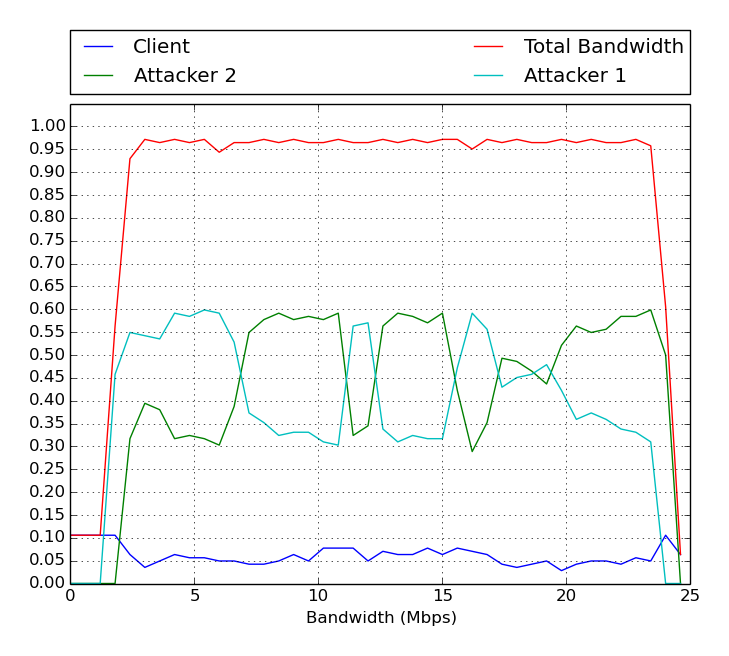
\includegraphics[width=0.5\textwidth]{../Results/tbf.png} \caption{DDoS attack on a DropTail queue.} \label{tbf1}
\end{figure}

\section{Results}

Figure \ref{tbf1} shows the bandwidth received by the client in one of the experiments under DropTail policy.
I was unable to verify that the client receive no bandwidth.
Instead, the experiment results in Figure~\ref{tbf1} show that the client experiences a noticeable rate drop.
The main reason for this discrepancy in my opinion is different implementation of Linux's Token Bucket Filter to NS2's DropTail policy. With TBF, tokens are generated at the given rate, and whenever one becomes available the first packet to arrive at the router will be forwarded. Therefore in real life implementation there's no way to drop all packets from the client, rather, the client will receive its fair share of bandwidth at the steady state. My experiment runs for 25 seconds and we may not reach steady state in this period.

\begin{figure}[b!]
    \centering
    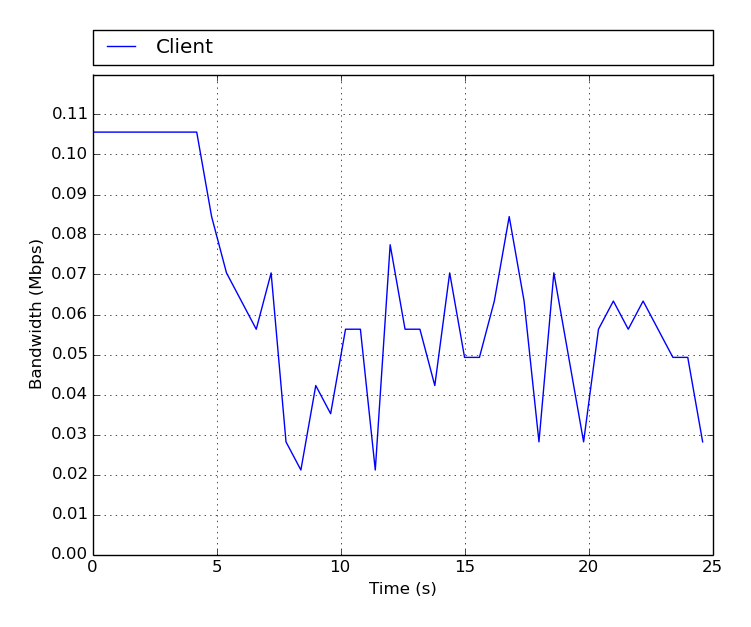
\includegraphics[width=0.5\textwidth]{../Results/red_client.png} \caption{Client bandwidth while RED router is DDoS'ed.} \label{red1}
\end{figure}

Figure \ref{red1} shows the bandwidth received by the client in one of the experiments under RED policy.
As expected and observed by the original paper, under RED we experience rate drop, similar phenomena is observed in my experiment, and for Figure 5 of the original paper, I can verify the result.
The experiment results in Figure~\ref{red1} show that the client maintains connectivity under RED even though attackers flood 9Mbps of packets to the router

\begin{figure}[t!]
    \centering
    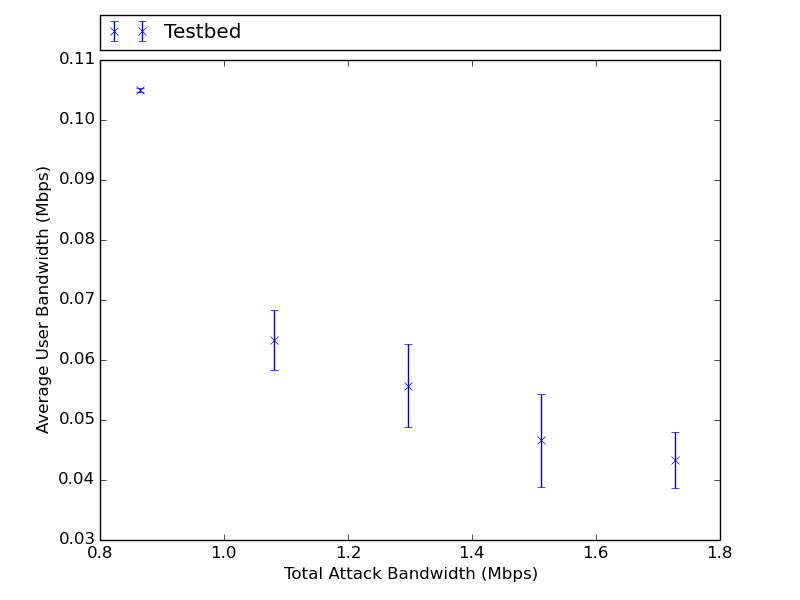
\includegraphics[width=0.5\textwidth]{../Results/result-tbf.png} \caption{Sensitivity analysis for DropTail queues.} \label{tbf2}
\end{figure}

Further, I also analyzed how sensitive these results are to change of total attack bandwidth.

As shown in Figure~\ref{tbf2}, under Token Bucket Filter queue, attackers can further degrade the client's desired rate by flooding more data.
At the steady state, we expect the client to receive its fair share of total bandwidth, although this experiment is too short, this plot verifies what we expect.

Under RED however, Figure~\ref{red2} shows that increasing total attack bandwidth does not affect the user by a noticeable margin and the client receives more than its fair share.
I expected the client to still receive its fair share under RED when the queue is overwhelmed.
Since when we send CBR UDP traffic, an overloaded RED queue is no different than a Token Bucket Filter.
However, we do not observe this phenomena here, and the client is receiving more bandwidth than its fair share.
I believe that the short duration of experiment is the main reason for this.
Note that for RED, we have setup a larger buffer compared to TBF, and hosts are at higher rates. Therefore it takes longer for the queue to reach its steady state and what we measure in Figure~\ref{red2} is essentially transient. Hence the poor correlation.

However, keep in mind that the original purpose of this experiment is to show that DDoS \emph{CAN} disrupt the clients demand. We did not design this experiment to compare RED and TBF in terms of fairness, and I have only addressed this issue since we talked about it during the presentation.
To compare the fairness, we need to modify this experiment, or at the very least make it last longer to let the queues reach their steady state.
But the main point of this experiment on DDoS attacks remains valid and we have shown how DDoS can disrupt queuing systems.
Also, the main point I wanted to make still stands: larger attack bandwidth further degrades quality of service for the client.

\begin{figure}[t!]
    \centering
    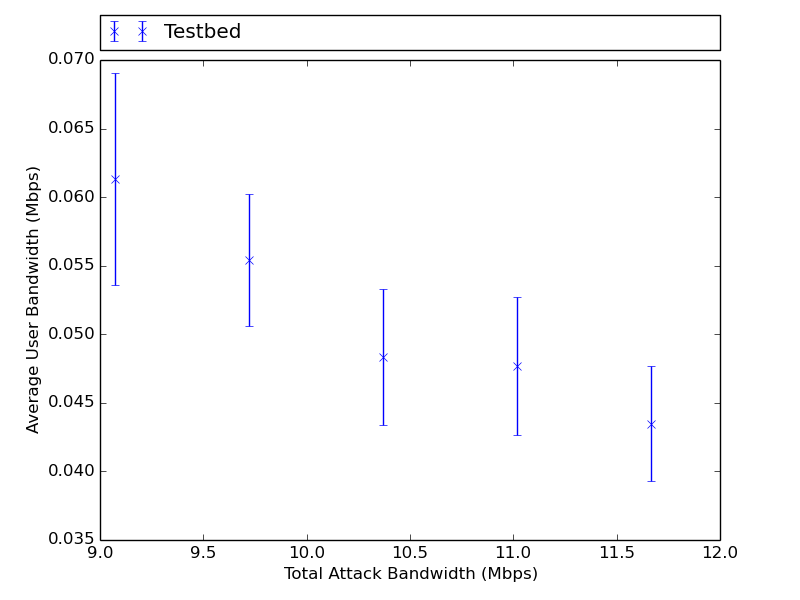
\includegraphics[width=0.5\textwidth]{../Results/result-red.png} \caption{Sensitivity analysis for RED queues.} \label{red2}
\end{figure}

\bibliographystyle{plain}
\bibliography{ref.bib}

\end{document}
